\chapter{Argumentación}\label{chapter:argumentation}

% Argumentacion background

\section{Argumentación}

La argumentación es el proceso que consiste en producir elementos que justifiquen una afirmación. Una afirmación 
constituye una expresión de algo ocurrido, un juicio, una evaluación. Las premisas son los elementos que 
justifican o atacan las afirmaciones. Un argumento básico está dado por la relación entre una afirmación y una 
premisa, con dicha premisa estar atacando o apoyando la afirmación inicial. Un ejemplo básico constituye:

\begin{center}
    "\emph{Las vacunas previenen la diseminación de enfermedades}, por lo tanto \textbf{vacunarse es necesario}."
\end{center}

En el ejemplo se puede observar un argumento simple y algunas características propias de estos, la justificación 
(en \textbf{negro}) que apoya la afirmación (en \emph{itálico}), también se puede observar palabras conectoras 
que indican además de conexión la dirección de esta.

Sobre esta han surgido diferentes marcos teóricos que buscan una metodología para su representación y estudio. 
Una de las más citadas constituye el Método o Modelo de Toulmin.

El Método Toulmin fue extrapolado del libro \emph{The Uses of Argument}[\cite{toulmin_2003}] escrito por Stephen E. Toulmin.
Este método divide los argumentos en seis partes: afirmación (claim), fundamento (grounds), 
justificación (warrant), calificador (qualifier), refutación (rebuttal) y respaldo (backing).
Mediante las afirmaciones se conoce el argumento principal que el autor quiere probar a la audiencia,
estas son respaldados con fundamentos siendo estos las evidencias y hechos en que se apoya el autor.
Las justificaciones pueden estar explícitas o implícitas y son suposiciones que vinculan los
fundamentos con las afirmaciones, estas a su vez pueden ser respaldadas por conocimiento.
El esquema introduce la posibilidad de otra sitaución válida a la establecida en las afirmaciones
mediante la refutación. Los calificadores son usados para dar más información de la calidad o seguridad
de las afirmaciones dadas. Un ejemplo de este esquema es:

\emph{[Se escucharon ladridos y aullidos en la distancia](fundamento), [probablemente](calificador) 
[haya perros en las cercanías](afirmación).}

En este ejemplo, además de las partes explícitas, se encuentran implícitas, la justificación 
(los perros son animales que ladran y aullan), el respaldo (se sabe que existen perros en la zona) y 
la refutación (Puede ser que hayan lobos o coyotes cerca). [\cite{toulminArgument}]
  
\section{Extracción de Argumentos}

El Procesamiento de Lenguaje Natural (\textbf{NLP} por sus siglas en inlgés \emph{Natural Language Processing}) es un 
subcampo de la Inteligencia Artificial (IA) que tiene como objetivo la comprensión del lenguaje humano por 
las computadoras. 
Mediante el uso de sus algoritmos es posible el procesamiento masivo de texto para la extracción de información 
relvante de este. Entre las tareas pertenecientes a dicho campo se encuentran Traducción Automática, 
Generación de Lenguaje Natural y Extracción de Argumentos (EA). La EA constituye la identificación y extracción 
automática de las estructuras de inferencia y 
razonamiento expresadas como argumentos presentes en el lenguaje natural [\cite{lawrence2020argument}].
En la actualidad en tareas de \textbf{NLP} como análisis de sentimientos permiten 
extraer cuales son las opiniones o sentimientos presentes, este análisis, sin embargo, presenta una falta 
de información, ya que no presenta el porqué de estas. La EA permite dar respuesta a este problema presentando
los argumentos y cómo sus relaciones justifican sus posiciones.

\subsection{Estructuras Argumentativas}

Las estructuras argumentativas son las partes y sus relaciones de las cuales están compuestas la argumentación en los textos.
Estas se componen de dos elementos principales, las Unidades de Discurso Argumentativas (UDA) y los enlaces
existentes entre estas. Las UDA presentan varias definiciones en las que se ven como cláusulas, oraciones, aunque
todas estas se presentan como secciones consecutivas de texto que no se sobreponen. Estas UDAs se relacionan entre 
sí formando el proceso de inferencia y razonamiento.
Tanto los enlaces como las UDAs son clasificadas en dependencia de su rol en la argumentación, estas clasificaciones 
parten de los conceptos de premisa y afirmación para las UDA y ataque y apoyo para las relaciones. 

\subsection{Tareas de extracción de argumentos}

Dada las estructuras argumentativas en la EA se conciben las siguientes tareas principales:

\subsubsection{Extracción de UDAs}

Esta tarea constituye en la separación de los segmentos de texto que formarán parte de la estructura.
El texto entrado es segmentado y como salida se obtiene un conjunto de UDAs. En el siguiente ejemplo se 
pone un ejemplo de la extracción de UDA (en \emph{itálico}).

\begin{center}
    Existen muchos efectos de la expansión de la tecnología en la transportación y las comunicaciones, 
    las cuales son mencionanadas ahora. En primer lugar, \emph{el correo electronico puede contar como uno de los resultados
    más beneficiosos de la tecnología moderna}. \emph{Años atrás, las personas pagaban gran cantidad de dinero para 
    enviar sus cartas y sus pagos estaban sujetos al peso de sus cartas o paquetes y muchos accidentes podrían 
    causar problemas que causarían que el correo no fuera enviado}.
\end{center}

\subsubsection{Clasificación de UDAs}

La clasificación de UDAs consiste en asignarle el papel que toma la UDA en la argumentación. En general 
las clasificaciones parten de dos clases bases, las afirmaciones, las cuales son posiciones que toma el 
autor del texto y las premisas, que son datos, eventos, elementos que se consideran verdades por sí solas.  

\begin{center}
    Existen muchos efectos de la expansión de la tecnología en la transportación y las comunicaciones, 
    las cuales son mencionanadas ahora. En primer lugar, \emph{el correo electronico puede contar como uno de los resultados
    más beneficiosos de la tecnología moderna}$_{Afirmación}$. \emph{Años atrás, las personas pagaban gran cantidad de dinero para 
    enviar sus cartas y sus pagos estaban sujetos al peso de sus cartas o paquetes y muchos accidentes podrían 
    causar problemas que causarían que el correo no fuera enviado}$_{Premisa}$.
\end{center}

\subsubsection{Extracción de relaciones entre las UDAs}

La extracción de relaciones constituye en determinar si estan relacionadas las UDAs. La disposición de estas
relaciones forma el proceso de razonamiento en que se basa el autor para validar su posición. En el ejemplo 
se representa la existencia de relación mediante su distancia argumentativa con la UDA con la que se relaciona.
La distancia argumentativa son la cantidad de UDAs del texto que separan la UDA fuente del objetivo [\cite{galassi2018argumentative}], 
en caso de ser negativa el objetivo se encuentra antes que la fuente y viceversa.

\begin{center}
    Existen muchos efectos de la expansión de la tecnología en la transportación y las comunicaciones, 
    las cuales son mencionanadas ahora. En primer lugar, \emph{el correo electronico puede contar como uno de los resultados
    más beneficiosos de la tecnología moderna}$_{Afirmación}$. \emph{Años atrás, las personas pagaban gran cantidad de dinero para 
    enviar sus cartas y sus pagos estaban sujetos al peso de sus cartas o paquetes y muchos accidentes podrían 
    causar problemas que causarían que el correo no fuera enviado}$_{Premisa, -1}$.
\end{center}

\subsubsection{Clasificación de relaciones entre las UDAs}

Los tipos de relaciones, nacen de dos clases bases por lo general, están las relaciones de apoyo y las de ataque.
Las de apoyo se centran en aquellas en las que la UDA fuente afirme la UDA objetivo, las de ataque se basan en 
las que la UDA fuente apoye la negación de la UDA objetivo.

\begin{center}
    Existen muchos efectos de la expansión de la tecnología en la transportación y las comunicaciones, 
    las cuales son mencionanadas ahora. En primer lugar, \emph{el correo electronico puede contar como uno de los resultados
    más beneficiosos de la tecnología moderna}$_{Afirmación}$. \emph{Años atrás, las personas pagaban gran cantidad de dinero para 
    enviar sus cartas y sus pagos estaban sujetos al peso de sus cartas o paquetes y muchos accidentes podrían 
    causar problemas que causarían que el correo no fuera enviado}$_{Premisa, -1 \space\space apoyo}$.
\end{center}

Partiendo de esto, se puede observar que las estructuras argumentativas de un texto constituyen un grafo dirigido 
en donde sus nodos representan las UDA y están anotados con su tipo y sus vértices representan las 
relaciones entre las UDA y dichos vértices se anotan con el tipo de relación existente entra ambas.

\begin{figure}[h!]
	\begin{center}
		\begin{center}
			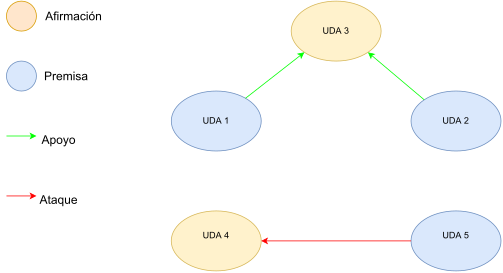
\includegraphics[scale=.3]{Graphics/Estructuras_argumentativas.png}
            % \includesvg[options]{Graphics/Estructuras argumentativas.svg}
        \end{center}
	    \caption{Estructuras Argumentativas}\label{fig:arg_struct}
	\end{center}
\end{figure}

\section{Preliminares de Extracción de Argumentos}

Varias investigaciones y propuestas han salido para dar respuesta a los problemas asociados a EA, mostrando
una variedad en enfoques y métodos.

En [\cite{palau2009argumentation}] se propone
el uso de modelos estadísticos como \emph{Naive Bayes} (\textbf{NB}) y \emph{Support Vector Machines} (\textbf{SVM}) 
para la clasificación de 
oraciones en argumentativas o no y en su rol argumentativo en caso de que sea argumentativa, en este
caso se asume que las componentes argumentativas son oraciones completas. Para la predicción de relaciones
se usa un enfoque basados en reglas con la creación de una Gramática Libre de Contexto. Las representaciones
de las oraciones se ven dadas por atributos creados a mano, dado el conocimiento experto sobre la argumentación
en el tema tratado, elementos como adverbios, verbos, signos de puntuación, palabras clave, estadísticas del texto
(Tamaño de oración, distancia media de palabras) son usados para la extracción y clasificación de las UDA, además
se usan también como base en la creación de las relgas de la gramática para la extracción de relaciones.

[\cite{goudas2015argument}] al igual que [\cite{palau2009argumentation}] clasifica las oraciones como
argumentativas o no mediante el uso de diferentes clasificadores como \textbf{NB}, \emph{Random Forest}, Regresión
Logística y \textbf{SVM}. En este trabajo se aumenta la grandularidad de la segmentación al permitir
la extracción de los segmentos que contienen la carga argumentativa de dentro de las oraciones previamente clasificadas
como tal, esto se realiza mediante la extracción de etiquetas BIO de las oraciones con el uso de un 
\emph{Conditional Random Field} (\textbf{CRF}). La predicción de las relaciones es modelado como un problema de clasificación
usando \emph{Support Vector Machine} para clasificar pares de UDA en relacionados o no. Atributos creados a mano 
son usados en la extracción de UDA entre estos están posición de la oración en el texto, cantidad de verbos, comas, adverbios,
palabras, entidades en la oración, también se emplean gaceteras que guardan entidades relacionadas con el dominio 
específico y palabras clave indicadoras de frases argumentativas. 

[\cite{stab2017parsing}] propone un mecanismo de segmentación basado en \textbf{CRF}. La clasificación
y predicción de relaciones es modelado conjuntamente como con dos clasificadores \textbf{SVM} y un problema
de Optimización Lineal Entero que encuentra la mejor estructura y asegurar una disposición arborea. En la segmentación
de las UDA se extraen por cada token su posición en el texto, si precede o sucede a un signo de puntuación, su parte de
la oración, la probabilidad de que sea el comienzo de una UDA dado sus tokens anteriores, entre otros. Para la extracción
y clasificación de relaciones se proponen otros conjuntos de atributos como la cantidad de sustantivos comunes entre
las componentes fuente y el objetivo, la presencia de indicadores argumentativos, representaciones vectoriales de tokens.

En [\cite{eger2017neural}] se enfocaron en presentar el problema de EA como uno \emph{end-to-end}. 
Para esto presentaron varias propuestas, entre ellas se encontraba
modelar el problema como un uno de secuencia a secuencia, usando Redes Neuronales Recurrentes (\textbf{RNN}) como 
\emph{Long-Short Term Memory} (\textbf{LSTM}) en versiones bidireccionales capturando información desde ambos lados de la secuencia,
para la representación de las palabras se extrajo información morfológica de las palabras mediante Redes Neuronales Convolucionales,
al final realizan la clasificación de la secuencia con un \textbf{CRF}. 
Realizaron experimentos al modelar el problema como uno de \emph{Dependency Parsing} en [\cite{kiperwasser2016simple}]. Este problema
consiste en construir un árbol de dependencia que codifique las estructuras argumentativas, en este problema 
se tiene que decidir entre varias opciones (\emph{shift}, \emph{reduce}) en dependencia del contenido de la pila y en el buffer.
El problema fue modelado también como un problema de reconocimiento de entidades nombradas, en donde las entidades son las UDA.

[\cite{galassi2018argumentative}] propone el uso de redes residuales y en combinación con mecanismos de atención
para la creación de un modelo el cual, conjuntamente, clasifica el tipo de UDA y la relación existentes entre estas.
Este trabajo define el concepto de distancia argumentativa, añadiéndolo como feature y asume que las UDA ya fueron 
extraídas. En este caso además de la distancia argumentativa las secuencias son representadas por sus representaciones
vectoriales de \textbf{GloVe}. Este trabajo asume la previa extracción de las UDAs.

En [\cite{dykes2020reconstructing}] se propone métodos basados en reglas para la extracción de argumentos sobre
textos en Twitter, estos métodos se centran en la confección de reglas basadas en anotaciones lingüísticas como
partes de la oración, lemas de palabras. La recuperación está basada en los esquemas argumentativos comunes presentes
en los textos. Este método apunta a una mayor precisión prescindiendo de recobrado. Dada las reglas creadas y el tipo
de datos con que se trabaja, cadenas de texto pequeñas, estos algoritmos tienden a tener una alta precisión aunque 
bajo recobrado, esto en conjuntos de datos grandes no es un gran problema, pero en conjuntos de menor tamaño o estructura 
más compleja pierden efectividad.

Se contempan disímiles enfoques al problema de EA desde una perspectiva enmarcada en modelos 
simbólicos, estadísticos y neuronales en versiones tanto secuenciales como \emph{end-to-end}. 
Cada uno de estos modelos presentan sus ventajas y desventajas a la hora de contruirlos, 
extenderlos y comprender su funcionamiento. En modelos simbólicos se presenta una alta
precisión en dominios específicos debido a que estos se construyen teniendo en cuenta reglas específicas a un
contexto dado. Estos modelos son poco escalables y difíciles de mantener ya que son sus reglas son construídas
a mano y dicho proceso requiere de conocimiento experto y tiempo. Modelos estadísticos son
característicos de usar conjuntos de atributos creados a mano, dichos atributos son difíciles
de encontrar, calcular y pueden no poseer relevancia en otros contextos diferentes a los que fueron creados. 
Además la necesidad de conocimiento experto es necesaria para su confección. Los modelos neuronales poseen
un mayor poder de adaptabilidad, en estos la entrada es codificada en una representación que es aprendida por
el mismo algoritmo, permitiendo seguir viable para distintos esquemas argumentativos. Los modelos simbólicos y 
estadísticos poseen la ventaja de poder explicar el porqué de los resultados devueltos cosa que se vuelve casi
imposible en modelos neuronales.

Dado que la EA es un proceso en el cual se necesita pasar por varias tareas, estas deben de ser completadas
de alguna forma. Una manera de completarlas es hacerla una a la vez, independiente una de otra y pasándole
la salida de etapas anteriores a las etapas siguientes. Esta manera secuencial de realizar las 
tareas es bastante simple y ayuda a la creación de modelos simples y con tareas bien definidas, aunque trae consigo 
la propagación de los errores a través del proceso y el no aprevechamiento de las interrelaciones entre variables 
computadas de procesos anteriores. Modelos \emph{end-to-end} en cambio poseen la habilidad de modelar el problema 
desde su inicio hasta su final de manera conjunta, mediante \emph{Multi-Task Learning} (\textbf{MTL}) se modelan
las tareas de manera conjunta creando modelos complejos aunque con una propagación de error menor.

% TODO?? Analisis de los resultados. Dado que los corpus son diferentes se ponen los mejores resultados encontrados
% por corpus y tambien de paso algunas métricas
